\documentclass[a4paper,12pt]{article}

\usepackage{ProfModels}
\usepackage{fig3d}
 
 
\begin{document}
\begin{Maquette}[DM]{Niveau=2, Numero=6, Date=19/10/2024, FinDate=31/12/2024, Semestre=2}


\begin{exercice}
\begin{enumerate}
\begin{minipage}{.55\linewidth}
Le tableau suivant représente le nombre d'enfant par famille.
\item compléter le tableau
\item Quel est le caractère de cette série statistique ?
\item Quel est l'effectif total de cette série statistique?
\item Calculer la moyenne de cette série statistique.
\item Tracer le diagramme en bâtons des effectifs.
\end{minipage}
\begin{minipage}{.45\linewidth}
\begin{tabular}{|Oc|Oc|Oc|Oc|Oc|Oc|}
\hline 
Nombre d'enfant & 1 & 2 & 3 & 4 & 5 \\ 
\hline 
nombre de famille & 3 & 10 & 7 & 4 & 8 \\ 
\hline 
Effectif cumulé  &  &  &  &  &  \\ 
\hline
Fréquence  &  &  &  &  &  \\ 
\hline 
Fréquence cumulé  &  &  &  &  &  \\ 
\hline
pourcentage &  &  &  &  &  \\ 
\hline 
\end{tabular} 
\end{minipage}
\end{enumerate}
\end{exercice}

\begin{exercice}
\begin{enumerate}
\begin{minipage}{.6\linewidth}
Voici la liste des notes d'un devoir de mathématiques 
\item compléter le tableau ci-dessous.
\item Calculer la moyenne de cette série statistique.
\item Donner le pourcentage des élèves qui ont obtenue la moyenne.
\item Représenter le tableau par un histogramme.
\item Représenter le tableau par un diagramme circulaire .
\end{minipage}%
\begin{minipage}{.4\linewidth}
\begin{tabular}{Oc|Oc|Oc|Oc|Oc|Oc|Oc|Oc}
12 & 15 & 14 & 8 & 6 & 8 & 14 & 14	 \\ 
\hline 
14 & 12 & 8 & 6 & 3 & 8 & 14 & 15	 \\ 
\hline 
12 & 8 & 6 & 6 & 3 & 8 & 14 & 15	 \\ 
\hline 
14 & 15 & 12 & 8 & 8 & 3 & 3 & 15 \\ 
\hline 
20 & 20 & 6 & 6 & 3 & 3 & 8 & 9 \\ 
\hline 
8 & 6 & 8 & 8 & 8 & 14 & 12 & 2 \\ 
\end{tabular} 
\end{minipage}%

\begin{tabular}{|Oc|Oc|Oc|Oc|Oc|}
\hline 
Classe : note  & $2\leq n < 6$ & $6\leq n < 10$ &$10\leq n < 16$ & $16\leq n \leq 20$ \\ 
\hline 
Nombre des élèves &  &  &  &  \\ 
\hline 
Effectif cumulé &  &  &  &  \\ 
\hline
Fréquence &  &  &  &  \\ 
\hline 
Pourcentage &  &  &  &  \\ 
\hline 
Mesure des angles &  &  &  &  \\ 
\hline 
\end{tabular} 
\end{enumerate}
\end{exercice}

\begin{exercice}
On considère le tableau de proportionnalité suivant :
\begin{tabular}{|*5{Oc|}}
\hline 
3 &  & 7 &  & 5 \\ 
\hline 
12 & 45 &  & 15.5 &  \\ 
\hline 
\end{tabular} 
\begin{enumerate}
\item calculer le coefficient de proportionnalité .
\item compléter le tableau 
\end{enumerate}
\end{exercice}


\begin{exercice}
Un TGV roule pendant 90 min  à la vitesse de 300 km/h.

Quelle distance parcourt-il ?
\end{exercice}

\begin{exercice}
\begin{enumerate}
\fullwidth{Aprés une remise de 135DH , un costume coûte 765DH.}
\item  De quel pourcentage son prix a-t-il diminué ?
\fullwidth{ Sachant que l'on a fixé une solde de -30\% sur un article coûte 480DH.}
\item Quel est le prix à payer ?
\end{enumerate}
\end{exercice}

\begin{exercice}
On considère la fonction linéaire $f$ tel que $f(x)=-3x$.
\begin{enumerate}
\item Calculer $f(3)$, $f(-1)$ et $f(\dfrac{2}{3})$.
\item Quel nombre a pour image -18 par $f$.
\item Représenter graphiquement la fonction $f$.
\end{enumerate}
\end{exercice}

\begin{exercice}
On considère les solides ci-dessous

\begin{tikzpicture}
\cylindre[0.6]{2}{4}
\tkzDrawSegment(O,A)
\tkzLabelSegment[above=-2pt, pos=.5](O,A){$2$}
\tkzDrawSegment[dim={$5$,6pt,left=4pt}](C,C')
\end{tikzpicture}
\begin{tikzpicture}
\cube[30]{4}{2}
\tkzLabelSegment[pos=.5](A,B){$6$}
\tkzLabelSegment[pos=.5,left](A,D){$2$}
\tkzLabelSegment[pos=.5](B,F){$3$}
\end{tikzpicture}
\begin{tikzpicture}
\pyramide[50]{4}{90}{50}
\tkzMarkRightAngle(S,A,B)
\tkzLabelSegment[pos=.5](A,B){$4$}
\tkzLabelSegment[pos=.5](B,C){$4$}
\tkzLabelSegment[pos=.5,left](A,S){$7$}
\end{tikzpicture}
\begin{enumerate}
\item Calculer le volume de chaque solide.
\item Calculer la surface latérale et totale du cylindre et du pavé.
\end{enumerate}
\end{exercice}

\end{Maquette}
\end{document}